\documentclass[a4paper, 12pt]{exam}

\usepackage[onehalfspacing]{setspace}
\usepackage{graphicx}
\usepackage{amsmath,amsfonts,amsthm,amssymb,mathtools}
\usepackage{nameref}
\usepackage{hyperref}
\usepackage{xcolor}
\usepackage{color,soul}
\usepackage{gensymb}
\usepackage[]{booktabs}
\usepackage[utf8]{inputenc}
\usepackage{array}
\usepackage{setspace}
\usepackage{verbatim} %for multiline comments https://tex.stackexchange.com/questions/44282/multiline-comment
\usepackage{xhfill}
\usepackage{enumitem}
\usepackage{varwidth}
\usepackage{multicol, array}
\usepackage{etoolbox}
\usepackage{multicol}
\usepackage[most,many,breakable]{tcolorbox}
\usepackage{mathtools}
\usepackage{background} %Package for adding a watermark
\usepackage{tikz-cd}
\usepackage{pgfplots} 
\pgfplotsset{compat=newest}
\usepgfplotslibrary{patchplots}
\usepackage{anyfontsize}
\usepackage{sectsty}
\usepackage[space]{grffile} %To allow for spaces in the path for the watermark
\usepackage{amsmath}
\usepackage{geometry} %lets us set the margins of the page
\usepackage{comment} %Allows for multi-line comments (\ifx \fi)
\usepackage{import} %lets us perform multi-file compilation
\usepackage{pdfpages} %allows for the inclusion of external multi-page PDF documents
\usepackage{algpseudocode} %lets you write algorithms (probably won't be used but i'm including it anyways) https://www.overleaf.com/learn/latex/Algorithms
\usepackage{bookmark}
\usepackage{theorem}

\usepackage{caption}


\usetikzlibrary{arrows, decorations.markings}
\usepackage{fontawesome}

\usetikzlibrary{hobby,backgrounds,positioning}
\usepackage{tikzsymbols}
\tikzsymbolsset{%
  after-symbol={},
}


\geometry{left=0.8in,top=0.5in, right = 0.8in}

\newcommand{\cuspac}{\hspace*{1cm}}

\backgroundsetup{contents=\includegraphics{Anant_Logo.png}, opacity=0.1, angle=0, scale=1.5}

\begin{document}
	\title{Anant 24-25 Recruitment Test}
	\author{Attitude Determination and Controls Subsystem (ADCS)}
	\date{January 18th, 2025}
	\maketitle
	
	\section*{Instructions}
	All general instructions are provided in the Google Classroom. Make sure you refer to them for submission details. Failure to adhere to the given rules may result in disqualification. 
	\begin{enumerate}[]
		\item This paper relies more on comprehension and general aptitude than it does in depth knowledge of the subject. You are encouraged to use the internet to solve this paper.
		\item Any changes to the paper will be posted in Google Classroom and an updated file will be shared. Please keep an eye out.
	\end{enumerate} 
	
	\bigskip

	\begin{enumerate}[label = \textbf{Rule \arabic* }:, leftmargin=5em]
		\item A student must prioritize developing an understanding of the topics being tested and demonstrating general aptitude, as evaluated during the subsequent interview where their solutions will be the main topic of discussion.
		
		\item A student must not collaborate with peers unless such collaboration is necessary to better achieve the goals outlined in Rule 1.
		
		\item A student must prioritize their physical and mental well-being, avoiding undue stress, all-nighters, or harmful study practices, unless doing so would conflict with Rules 1 or 2.
		
			\end{enumerate}
		
If you have any questions regarding the content of the paper, feel free to reach out to any of the undersigned for help. \\

Contact Details:
		\begin{enumerate}
			\item Aaditya Thakkar - +91 81282 17114
			\item Nikhil Mathew - +91 97400 44411
			\item Pranav Chandra - +91 90807 96426
			\item Pramit Pal - +91 99026 97222
		\end{enumerate}

	\begin{center}
		\textbf{All the best!}
	\end{center}
		
	\pagebreak
	
	\newgeometry{left=0.75in,top=1in, right = 0.75in}


\section*{Question 1: The hunt for the cosmic herb}

\noindent \textit{Scene opens with Rick scribbling frantically on an old map while Morty nervously watches from the side.}

\bigskip
\noindent \textbf{Rick:} “Morty! MOR-TY! Look at this treasure! Found it in some dusty drawer in my lab. This map leads to what’s described as the finest plant-based relaxation on Earth—none of that store-bought junk, Morty. This is the real deal! Some cosmic entity mapped this out, pointing to $(3182.655, 2000.94, 5135.159) \ \mathrm{km}$ back on January 3, 1920, at 1420 VLAT—don’t give me that look, Morty. It’s UTC+10:00, keep up!” \\

\noindent \textbf{Morty:} “Wait, what are you even talking about, Rick? Why does the map matter? Can’t we just, like, drive there?” \\

\noindent \textbf{Rick:} “Oh, yeah, sure, Morty. Just drive there! Except this hill? Yeah, it’s in the middle of nowhere. And those coordinates? They’re in the Earth-Centered Earth-Fixed (ECEF) Frame. That means it’s tied to Earth’s rotation. The origin’s at Earth’s center of mass—big deal, right? You need to figure out the latitude, longitude, and altitude of this hill, Morty. Oh, and also tell me where on Earth this place actually is. Let’s get to work!” \\

\hl{$(a)$ Locate the hill using the ECEF coordinates $(3182.655, 2000.94, 5135.159) \ \mathrm{km}$. Find the latitude, longitude, and altitude. Also, determine the physical location (i.e., name of the place) on Earth.}

\bigskip
\noindent \textbf{(A few hours pass as Morty calculates furiously. Rick returns with a teleporter.)} \\

\noindent \textbf{Rick:} “Good news, Morty! We’ve got this celestial teleporter that came with the map. Bad news? The cosmic genius that built it didn’t account for Earth’s rotation. The teleporter only takes coordinates in the Earth-Centered Inertial (ECI) Frame. That’s a frame fixed to the stars, Morty. Conveniently, ECI and ECEF align perfectly at 1200 GMT every day. So, get to it—convert the hill’s coordinates to the ECI frame using today’s time.” \\

\noindent \textbf{Morty:} “So, uh, what do I need to do, Rick?” \\

\noindent \textbf{Rick:} “What do you need to do? Convert the coordinates! ECI frame, Morty. Use today’s date. We’re not waiting around forever.” \\

\pagebreak

\hl{$(b)$ Convert the hill's position into the Earth Centered Inertial Frame for today's date and time (Mention the time and date you used). Use the assumption that ECEF and ECI align perfectly at 1200 GMT daily.

[\textbf{Caution:} The assumptions in this question overly simplify reality. They may not necessarily match other res.]}


\bigskip
\noindent \textbf{(Morty does the conversion. They teleport, but end up in deep space.)} \\

\noindent \textbf{Rick:} “Morty! What did you do?! I told you to convert the coordinates properly, but you used Earth’s current position, didn’t you? Morty, the Earth back in 1920 was in a different position in space! The ECI frame is anchored to the stars, not Earth’s current rotation!” \\

\noindent \textbf{Morty:} “I-I didn’t think it would matter, Rick! I mean, how different could it—” \\

\noindent \textbf{Rick:} “Stop talking, Morty! Listen, the Earth’s position back in 1920 needs to be calculated based on its orbit around the Sun. Picture the Earth’s elliptical orbit. The $z$-axis is perpendicular to the orbital plane, lying in the positive $z$-half, and the $x$-axis points from the center of the ellipse to the aphelion. Got it?” \\

\noindent \textbf{Morty:} “Uh, not really...” \\

\noindent \textbf{Rick:} “Fine! I’ll calculate the Earth’s position in 1920 and compare it to now using celestial mechanics. Then you’ll re-convert those coordinates to the ECI frame for 1920 and plug them into the teleporter! Otherwise, we’re stuck here!” \\

\noindent \textbf{Rick:} “And hurry up, Morty! This cosmic herb isn’t going to find itself!” \\

\hl{$(c)$ Parameterize Earth's position in its orbit for January 3rd, 1920, at 1420 VLAT (UTC+10:00) such that the center of the orbital ellipse is the origin. Re-convert the hill's current position with respect to the ECI frame of January 3rd, 1920 and input them into the teleporter.}

	\pagebreak
	
	\section*{Question 2 - Forget Physics, We’re Reaching the Stars!}

\noindent \textbf{(Rick and Morty are still floating in space after Morty’s last mishap. Rick is furiously tinkering with the teleporter, while Morty nervously looks at the flashing “ERROR: COORDINATE MISMATCH” on the screen.)}

\bigskip
\noindent \textbf{Rick:} “Morty, I’m about two seconds away from strapping you to this teleporter and using you as an improvised space anchor! Do you have any idea how badly you messed up? We’re stuck out here in the middle of the cosmic void, Morty, and it’s up to you to fix it!” \\

\noindent \textbf{Morty:} “B-but Rick, I don’t even know what I did wrong! I just followed your instructions!” \bigskip

\noindent \textbf{Rick:} “Exactly, Morty! You followed without thinking. Fine, you want a way back? Time to do some orbital mechanics homework. Here’s your first problem!”

\bigskip

\noindent \textbf{Rick:} “Alright, listen up, Morty. There’s this planet over there, minding its business in a nice circular orbit, and we’re in another circular orbit. To get there, we need to perform some clever orbital maneuvers. No teleporters, no shortcuts, no fancy tricks—just good old-fashioned physics. Figure out the two burns we need to transfer from our orbit to theirs.”

\bigskip

\hl{$(a)$ Calculate the $\Delta V$ required for both burns to transfer from an orbital altitude of 200 km to 2000 km.}

\begin{center}
	\begin{tikzpicture}[ scale=1.50,
    >=triangle 45,
    mydeco/.style = {
        decoration = {
            markings, 
            mark = at position #1 with {
                \node[scale=1.2, rotate=\pgfdecoratedangle+140] {\faRocket};
            }
        }
    }
]
                      
         \draw (-1,-0.165) node[rotate=180, color=orange, scale = 1.5] {\Fire};
    \draw (-1.05,0) node [anchor = east, scale = 0.75, color=orange]  {$1^{st} \ Burn \ \ $};
    \draw (2.5,0.05) node[rotate=0, color=orange, scale = 1.5] {\Fire};
    \draw (2.5,0) node [anchor = east, scale = 0.75, color=orange]  {$2^{nd} \ Burn \ \ $};                 
                      
    \filldraw[top color = blue!75!green, bottom color = blue!60, opacity = .75] (0,0) circle (.5cm);
    
    \draw[postaction = {mydeco=-0.2416 ,decorate}, 
          postaction = {mydeco=-0.58333 ,decorate},
          postaction = {mydeco=-0.0075 ,decorate}]
          (0,0) circle (2.5cm);

    \draw[postaction = {mydeco=-0.375 ,decorate}, 
          postaction = {mydeco=-0.875 ,decorate}] (0,0) circle (1cm);
    \draw (0.65,-1.2) node [anchor = east, scale = 0.8]  {Initial Orbit};
    

    \draw[postaction = {mydeco=0.5 ,decorate, color=black}, 
          postaction = {mydeco=0.9975 ,decorate, color=black}, color = orange, thick] (0:2.5) arc (0:180:1.75cm and 1.3cm);
     \draw (0.65,2.7) node [anchor = east, scale = 0.8]  {Final Orbit};
    



	\end{tikzpicture}
	\end{center}


\noindent \textbf{Rick:} “Here’s a visual aid for you, Morty, since your brain can’t handle too many variables. Now get to work!”

\bigskip
\noindent \textbf{Rick:} “Good job, Morty! You managed to figure out the basic transfer orbit. Congratulations, you’re officially smarter than a potato. But now, let’s make this interesting. Sometimes, instead of taking the direct route, it’s better to take a detour. That’s right, Morty—go out to a higher orbit first, then come back down to your target. Think of it like taking a scenic route, except it’s all about saving fuel, not enjoying the view.”

\bigskip

\noindent \textbf{Morty:} “Wait, Rick, why would going farther out save fuel? Doesn’t that seem like a waste?” 

\bigskip

\noindent \textbf{Rick:} “Oh, Morty, sometimes I wonder how you even manage to function. Look, going farther out can give you a better angle or reduce energy losses. I’m not here to explain the ‘why’—just do the math! Three burns this time: one to leave the starting orbit, one to reach the higher orbit, and one to finish at the target. Figure it out!”

\bigskip

\begin{center}

\begin{tikzpicture}[ scale=1.750,
    >=triangle 45,
    mydeco/.style = {
        decoration = {
            markings, 
            mark = at position #1 with {
                \node[scale=1.2, rotate=\pgfdecoratedangle+140] {\faRocket};
            }
        }
    }
]
                      
        \draw (-1,-0.15) node[rotate=180, color=orange, scale = 1.5] {\Fire};
    \draw (-1,0) node [anchor = east, scale = 0.75, color=orange]  {$1^{st} \ Burn \ \ $};
    \draw (5,0.15) node[rotate=0, color=orange, scale = 1.5] {\Fire};
    \draw (5,0) node [anchor = east, scale = 0.75, color=orange]  {$2^{nd} \ Burn \ \ $};
    \draw (-2.5,-0.165) node[rotate=180, color=orange, scale = 1.5] {\Fire};
    \draw (-2.5,0) node [anchor = east, scale = 0.75, color=orange]  {$3^{rd} \ Burn \ \ $};
    
    \filldraw[top color = blue!75!green, bottom color = blue!60, opacity = .75] (0,0) circle (.5cm);
    
    \draw[ color = teal] (0:5) arc (0:-180:3.75cm and 3.2cm);
    %\draw[ color = teal, dashed] (0:5) arc (0:180:3.75cm and 3.2cm);
    \draw (2,-3.35) node [anchor = east, scale = 0.8, text=teal]  {Transfer Orbit 2};
    
        \draw[ 
          postaction = {mydeco=0.9975 ,decorate, color=black},postaction = {mydeco=0 ,decorate, color=black}, color = orange] (0:5) arc (0:180:3cm and 1.7cm);
         % \draw[color = orange, dashed] (0:5) arc (0:-180:3cm and 1.7cm);
          \draw (3.5,1.8) node [anchor = east, scale = 0.8, text=orange]  {Transfer Orbit 1};
 
    
    \draw[postaction = {mydeco=-0.2416 ,decorate}, 
          postaction = {mydeco=-0.68333 ,decorate},
          postaction = {mydeco=-0.5 ,decorate},]
          (0,0) circle (2.5cm);

    \draw[postaction = {mydeco=-0.15 ,decorate}, 
          postaction = {mydeco=-0.75 ,decorate}] (0,0) circle (1cm);
    \draw (1.65,-1) node [anchor = east, scale = 0.8]  {Initial Orbit};
    


          
          
          
     \draw (1.65,2.55) node [anchor = east, scale = 0.8]  {Final Orbit};
    

    


	\end{tikzpicture}
\end{center}

\hl{$(b)$ Calculate the $\Delta V$ required for three burns in this new transfer orbit to go from 200 km to 2000 km. Compare it to the transfer in part $(a)$ and explain why it might be used.}

\bigskip

\noindent \textbf{(Morty scribbles furiously, enters coordinates, and then accidentally presses a big red button labeled \textcolor{red}{DO NOT PRESS}.)}

\bigskip

\noindent \textbf{Morty:} “Rick, what just happened?! What did I do?!” \\

\noindent \textbf{Rick:} “Oh, great, Morty, just great! We’ve landed in a universe where physics doesn’t play fair anymore. You know how gravity works with $F = G \frac{m_1 m_2}{r^2}$? Well, not here, Morty! Here, gravity scales with $r^{-3}$. Imagine that, Morty—a universe where the rules of nature decided to take a vacation!”

\bigskip

\noindent \textbf{Morty:} “R-rick, how does that even work? What happens to orbits here?” \\

\noindent \textbf{Rick:} “I don’t know, Morty! Do I look like a cosmic physicist? You need to figure it out. When gravity changes to $F \propto r^{-3}$, everything’s different—Kepler’s laws? Gone. Orbital mechanics? Completely reworked. What kind of orbits do we get, Morty? Are they stable? Do they spiral? Are they just chaos? It’s up to you to solve this before we float out here forever!”

\bigskip

\hl{$(c)$ Figure out how this changes the orbits and the maneuvers required to transfer between them.}

\bigskip

\noindent \textbf{Rick:} “Morty, if you don’t figure this out, I’m sending you to a universe where you’re the gravitational constant. Let’s see how you like being orbited by space debris for eternity.”

	
	\pagebreak
	

\section*{Question 3: Lost in space, betrayed by science (and worm goo)}

\noindent \textbf{(Morty is floating in space, clutching the half-broken GPS tracker that Rick gave him before they were separated. A flickering hologram of Rick appears, not looking pleased.)}

\bigskip
\noindent \textbf{Morty:} “Oh man, Rick! I-I don’t know where I am! One second we were fine, and then the worm sucked us into its dimension, and now I’m floating in space! HELP!” \bigskip

\noindent \textbf{Rick (Hologram):} “Morty, I told you not to mess with the worm! But nooo, you couldn’t help yourself. And now you’re stranded in deep space, tumbling around like a cosmic yo-yo. Fantastic, Morty. Just fantastic.” \bigskip

\noindent \textbf{Morty:} “I-I thought the worm was harmless, Rick! It was just sitting there glowing! You didn’t say it could explode into a vortex!” 

\bigskip

\noindent \textbf{Rick:} “Well, Morty, now you’re gonna have to use that barely-working GPS I gave you. It’s not much, but it’ll have to do. Alright, let’s start with something simple. The GPS tracker has a pinging system—it sends a signal to satellites, and they bounce it back. Basic physics, Morty. I gave you the coordinates of three satellites before you decided to mess everything up. Here they are:”

\begin{center}
Satellite A: (-3141, -5926, 5358) \\
Satellite B: (-9793, 2384, -6264) \\
Satellite C: (3383, -2795, -0288)
\end{center}

\noindent \textbf{Rick:} “But here’s the thing, Morty: there’s a fourth satellite I didn’t tell you about. Why? Because you need to learn to problem-solve, Morty! Here’s a hint: its \(x, y, z\) coordinates are symmetric—all the same value, \textbf{and} $x, y, z \leq 1000 km$” 

\bigskip
\noindent \textbf{Morty:} “B-but Rick, how am I supposed to figure out where I am?!” \bigskip

\noindent \textbf{Rick:} “Morty, are you even listening? I gave you the ping times for all four satellites. Here they are:”
\[
t_A = 47.81974730 \, \text{ms}, \quad t_B = 103.14672440 \, \text{ms}, \quad t_C = 43.58455434 \, \text{ms}, \quad t_D = 29.93312378\, \text{ms}.
\]

\hl{$(a)$ Using the provided data, calculate two things: $(i)$ Morty's position in space and $(ii)$ the coordinates of the fourth satellite.}

\bigskip

\noindent \textbf{(After managing to calculate his position and the missing satellite’s coordinates, Morty accidentally triggers the GPS’s emergency protocol. The tracker sparks violently and blurts out: \textcolor{red}{“WORM CONTAMINATION DETECTED! INITIATING SELF-CLEANSE!”})}

\bigskip

\noindent \textbf{Morty:} “AHHHHH! Rick! The GPS is going crazy!” 

\bigskip

\noindent \textbf{Rick (Hologram):} “Morty, you managed to infect the GPS with interdimensional worm goo. That’s impressive in the worst possible way. Now it’s purging itself, which means it’s gonna lose half its functionality. Luckily, you’ve still got data from three satellites. Make it work, Morty!” 

\bigskip

\noindent \textbf{(The GPS fires a small thruster, sending Morty hurtling uncontrollably through space. It spits out two sets of pings before breaking down completely.)}

\bigskip

\noindent \textbf{Rick:} “Alright, Morty, here’s the last bit of data the GPS managed to collect:”
\[
\begin{aligned}
A_1 &= 28.21941442 \, \text{ms}, & A_2 &= 32.56521822 \, \text{ms}, \\
B_1 &= 37.40539321 \, \text{ms}, & B_2 &= 37.48077648 \, \text{ms}, \\
C_1 &= 21.88477974 \, \text{ms}, & C_2 &= 35.47581482 \, \text{ms}.
\end{aligned}
\]

\noindent \textbf{Rick:} “Oh, and the timestamps? The first set is at \(t_1 = 0 \, \text{s}\), and the second set is at \(t_2 = 5000 \, \text{s}\). That’s 5000 seconds, Morty, because worm goo messes with everything. Using just these three satellites, calculate your direction vector and velocity. You’ve got this, Morty! (Probably.)”

\bigskip

\hl{$(b)$ Calculate all possible velocity vectors Morty may be taking using the distance data provided.}

\bigskip

\noindent \textbf{(After what feels like an eternity, Morty finally crash-lands into Earth’s orbit. He breathes a sigh of relief, but the GPS breaks apart, leaving him with a sun sensor and a magnetic field sensor.)} 

\bigskip

\noindent \textbf{Morty:} “Rick, the GPS is gone! What do I do now?!” 

\bigskip

\noindent \textbf{Rick (Hologram):} “Morty, you’ve still got a sun sensor and a magnetic field sensor. That’s enough to figure out your orientation relative to Earth. Tape the sensors to your chest if you have to, and send the data to ground control so they can save you!”

\bigskip

\hl{$(c)$ Explain how to use the sun sensor and magnetic field sensor to determine Morty's orientation relative to Earth. Include a sketch.}	
	
\pagebreak

\section*{Question 4: The final discovery}

\noindent \textbf{(Morty is standing in the middle of a dense jungle somewhere on Earth, after a chaotic adventure filled with worm goo, broken GPS systems, and intergalactic mishaps. His GPS is down to its last feature—a distance tracker—and Rick’s hologram flickers into life.)}

\bigskip
\noindent \textbf{Morty:} “Rick! I’m here in the middle of nowhere, but I don’t see the herb! I thought you said this was a treasure map or something! Where is it?!” \bigskip

\noindent \textbf{Rick (Hologram):} “Morty, I didn’t just say it was a treasure map—I meant it! The herb is right there, Morty! Somewhere in this jungle. But, surprise surprise, you’re too clueless to find it. Lucky for you, I left you one last device that can measure its distance. Quit whining and start using it!” \bigskip

\noindent \textbf{Morty:} “I-I don’t know, Rick. This jungle is huge! What do I do?” \bigskip

\noindent \textbf{Rick:} “What do you do now, Morty? You figure out where the herb is! Use the first \(n\) distance measurements to estimate its true position. This is math class now, Morty. Here’s what you’ve got so far:”

\[
(x_1, y_1), (x_2, y_2), \dots, (x_n, y_n)
\]

\noindent \textbf{Rick:} “Use this data to figure out where the herb actually is. And no, Morty, you can’t just walk around aimlessly—that’s inefficient and dumb! Calculate the true position using the measurements. Get to work!”

\bigskip

\noindent \textbf{Morty:} "Wha? Rick, but I can't! I don't know what to do!"

\bigskip

\noindent \textbf{Rick:} “Alright, Morty, let’s break it down. First, assume the herb isn’t moving. Use the first \(n\) measurements to estimate its actual location. If you don’t know how to do that, Morty, then maybe you should just quit and go home.”

\bigskip
\hl{$(a)$ Estimate the herb's true position: Use the first \textit{n} positions to calculate its actual location.}
\bigskip

\noindent \textbf{Rick:} “Obviously, manually calculating every position isn’t going to work. You need a formula, Morty—something that dynamically updates using the \(k\)$^{th}$ estimate and the \((k+1)\)$^{th}$ measurement. Less walking, more calculating!”

\bigskip
\hl{$(b)$ Derive a formula that uses the $k$$^{th}$ estimate and the $(k+1)$$^{th}$ measurement to refine the herb's position.}

\bigskip

\noindent \textbf{Rick:} “Now, let’s make it specific. These are the herb’s recorded positions as you’ve moved through the jungle:”

\[
\begin{aligned}
\{ 
&(-4.135, 2.81), \quad (-4.859, -1.178), \quad (-3.52, 3.551), \quad (-4.543, 2.088), \quad  (-4.185, 2.736), \\
&(-4.993, 0.269), \quad (-4.455, 2.27), \quad (-1.566, 4.748), \quad (-4.843, -1.243), \quad (-4.848, 1.222)
\}
\end{aligned}
\]

\noindent \textbf{Rick:} “Estimate the true position of the herb and calculate how far you are from it. Don’t mess this up, Morty! That herb isn’t going to magically appear in your hands!”

\bigskip

\hl{$(c)$ Use the provided measurements to estimate the herb's true distance from Morty.}
\bigskip

\noindent \textbf{(Morty finally calculates the herb’s position and starts moving towards it, but suddenly he hears rustling in the jungle.)}

\bigskip
\noindent \textbf{Morty:} “Rick! I think the herb is moving! What’s going on?!” \bigskip

\noindent \textbf{Rick:} “Of course it’s moving, Morty! Did you think it was just going to sit there? The herb isn’t a plant—it’s attached to a small animal, Morty! It’s a jungle critter carrying the herb and running in circles. You need to predict where it’ll go next! Using the first \(n\) measurements, calculate its next position. Hurry up, Morty!”

\bigskip

\hl{$(d)$ Assuming the herb is being carried in a circular path with a constant angular velocity $\omega \, \mathrm{rad/s}$, estimate the value of $\omega$ and where it will be at $t = t_k$.}

\bigskip
\noindent \textbf{Rick:} “Alright, Morty, let’s get real. These are the critter’s recorded positions over the last few seconds:”
\begin{align*}
\{
&(-4.349, 2.468), \quad (-4.789, 1.438), \quad (-4.898, 1.003), \quad (-4.741, 1.588), \quad (-4.92, 0.893), \\
&(-4.92, -0.893), \quad (-3.471, -3.598), \quad (1.373, -4.808), \quad (2.428, -4.371), \quad (4.315, -2.526)
\}
\end{align*}

\noindent \textbf{Rick:} “Predict where the herb will be at \(t = 5.5 \, \mathrm{s}\), Morty. Get your act together and figure it out!”

\bigskip

\hl{$(e)$ Predict the herb's location at $t = 5.5 \, \mathrm{s}$ based on the provided measurements.}
\bigskip

\noindent \textbf{(Morty finally calculates the herb’s position and manages to catch the critter carrying it just before it escapes. He breathes a sigh of relief as Rick’s hologram flickers back on.)}

\bigskip
\noindent \textbf{Morty:} “I-I did it, Rick! I got the herb! What do I do now?” \bigskip

\noindent \textbf{Rick:} “What do you do now, Morty? You enjoy the fruits of your labor! But, knowing you, you’ll probably trip and drop it in the mud. Just don’t lose it on the way back, Morty—I’ve had enough of this adventure!”

\bigskip

\noindent \textbf{(Morty groans as he starts his trek back to civilization, with Rick’s sarcastic commentary echoing in his ear.)}

\end{document}